% !TEX root = ../main.tex

\chapter{Experiments}
\label{ch:experiments}
This chapter aims to answer the research questions formulated in Section~\ref{sec:research_questions}. First, I describe which experiments I conducted. Next, I show the results of these experiments. Finally, I discuss my findings further in the last section.

\section{Reproduction of Previous Results}
For a starting point, I reproduced the results of the paper \emph{Analyzing Reinforcement Learning Benchmarks with Random Weight Guessing} (\cite{oller_analyzing_2020}) discussed in Section~\ref{sec:benchmarks}. I used the same methodology as the authors of the paper did. In specific, I used three network architectures: a network without any hidden layers (0 HL, 0 HU), a network with a single hidden layer of 4 units (1 HL, 4 HU), and a network with two hidden layers of 4 units each (2 HL, 4 HU). I used the same procedure as explained in pseudocode in Algorithm~\ref{alg:environment-evaluation} using RWG. I tested the three neural networks for all five classic control environments provided by the OpenAI Gym interface: \verb|CartPole|, \verb|Acrobot|, \verb|Pendulum|, \verb|MountainCar|, and \verb|MountainCarContinuous|. For the next experiments, the reproduced results serve as a baseline to judge the effectiveness of the alternative models in comparison with neural networks.

\subsection{Results}
Figure~\ref{fig:results_NN} shows the results for all five classic control environments using neural networks without bias.
\begin{figure}
  \centering
  \includegraphics[width=\linewidth]{NN/NN_CartPole_new}

      \vspace{0.2cm}

  \includegraphics[width=\linewidth]{NN/NN_Acrobot_new}

      \vspace{0.2cm}

  \includegraphics[width=\linewidth]{NN/NN_MountainCar_new}

      \vspace{0.2cm}

  \includegraphics[width=\linewidth]{NN/NN_MountainCarContinuous_new}

      \vspace{0.2cm}

  \includegraphics[width=\linewidth]{NN/NN_Pendulum_new}
\caption[Results for all classic control environments using neural networks without bias]{
  \textbf{Results for all classic control environments using neural networks without bias.}
   Each row shows the results of one environment, whereas the columns represent the different network architectures. These plots are a reproduction of the results of the RWG-paper. My results are consistent with those shown in the paper.
}
\label{fig:results_NN}
\end{figure}
For each plot, the samples are ranked according to their mean score and aligned on the $x-$axis according to their rank. The scatter plots show all scores of the samples, whereas the lineplot illustrates the mean of each sample over all episodes. Each column shows a different network architecture. The first column shows the results of the networks without hidden layers, the second column the networks with one hidden layer, and the last column the networks with two hidden layers. The rows are dedicated to the different classic control environments.

These results are consistent with the ones from the paper \emph{Analyzing Reinforcement Learning Benchmarks with Random Weight Guessing}. In the subsequent sections, I will refer to these plots to compare the effectiveness of other models or configurations to these neural network architectures.

\section{Comparison of Alternative Models to Neural Networks}
This experiment aims to provide a comparison of alternative models to the commonly used neural network model. I selected a few promising models and analyzed them with the help of the classic control environments. Analogous to the neural networks, I used three architectures for each model with increasing complexity. I conducted the following experiments:
\begin{enumerate}[label=(\alph*)]
  \item In the first experiment, I took the polynomial model $P_1$ and tested it on the discrete classic control environments. I used polynomials of degrees 1, 2, and 3.
  \item In the second experiment, I tested the binary tree model on all five classic control environments. I used binary trees with 1, 4, and 8 nodes.
\end{enumerate}
I described the models in more detail in Section~\ref{sec:environments}. For the experiments, I used the same procedure as in \emph{Analyzing Reinforcement Learning Benchmarks with Random Weight Guessing} with only slight adaption. Thus, we can directly compare the results of the alternative models to those of neural networks. Another important aspect of this procedure is that there is no learning involved. For their paper, the authors were interested in the complexity of the environment, whereas I aim to find out more about the nature of the models. The classic control environments are relatively easy to solve, as explained in Section~\ref{sec:benchmarks}. Therefore, we expect some controllers to solve the task even without any learning involved.

For the experiments, first, I initialized the environment. Second, I initialized the respective model. Then, I drew the weights of the model from the standard normal distribution $\mathcal{N}(0,1)$ or the uniform distribution $U(a,b)$ depending on the model and environment used. Each of these instances of the model represents a sample. In total, I used $10'000$ samples ($N_{samples}$). Finally, I ran 20 episodes ($N_{episodes}$) with each sample for an environment and stored the respective score as an entry of the score tensor $S$. Algorithm~\ref{alg:model-evaluation} shows an overview of the described procedure. As we can see, the procedure is very similar to the one shown in Algorithm~\ref{alg:environment-evaluation}.
\begin{algorithm}
\caption{Procedure for alternative models using RWG}
\begin{algorithmic}[1]
\State Initialize environment
\State Initialize model
\State Create array $S$ of size $N_{samples} \times N_{episodes}$
\For{$n = 1,2,...,N_{samples}$}
    \State Sample model weights randomly from $\mathcal{N}(0,1)$ or $U(a, b)$
    \For{$e=1,2,...,N_{episodes}$}
      \State Reset the environment
      \State Run episode with model
      \State Store accured episode reward in $S_{n,e}$
    \EndFor
\EndFor
\end{algorithmic}
\label{alg:model-evaluation}
\end{algorithm}

\section{Analysis of the Impact of Bias}
The authors of the paper \emph{Analyzing Reinforcement Learning Benchmarks with Random Weight Guessing} indicate that using bias worsens the performance of neural networks in their experimental setting. This experiment serves to analyze this behavior. I used the same procedure as explained in the paper with the same three neural network architectures: a network without any hidden layers (0 HL, 0 HU), a network with a single hidden layer of 4 units (1 HL, 4 HU), and a network with two hidden layers of 4 units each (2 HL, 4 HU). First, I reproduced the results for the networks with bias to confirm their findings. Then, I varied the number of (a) weights, (b) hidden layers, and (c) neurons for a neural network. To get insights into whether this observation is specific to neural networks, I additionally used the polynomial model for the experiment concerning the variation of the weights of the model. In more detail, the experiments I conducted in this matter are the following:
\begin{enumerate}[label=(\alph*)]
  \item In the first experiment, I only changed the number of weights for each of the three networks and the polynomial model $P_1$ described in Section~\ref{sec:models}. I tripled the number of weights for all models. To achieve this, I constructed one weight $\mathbf{w_i}$ out of three weights by addition:
  \begin{align*}
    &\text{Triple number of weights: } &\mathbf{w_{i}} &= \mathbf{w_{i1}} + \mathbf{w_{i2}} + \mathbf{w_{i3}}
  \end{align*}
  \item In the second experiment, I tested the neural network models with different numbers of hidden layers. Each layer still has the same number of hidden neurons as before. Thus, the networks have four hidden units for each layer. I analyzed a network with 4 hidden layers, one with 6, and one with 8.
  \item In the last experiment concerning this subject, I varied the number of hidden neurons for a network. Here, I only used a network with two hidden layers. For the number of hidden neurons, I chose 5, 8, and 10.
\end{enumerate}

\section{Polynomial Model}
Figure~\ref{fig:results_Polynomial} shows the results for the discrete classic control environments using the polynomial model $P_1$ without bias. The visualization is identical to the one I used for the neural networks in Figure~\ref{fig:results_NN}. The rows show the results for the different environments, and the columns show the polynomial with degrees 1, 2, and 3.
\begin{figure}[!ht]
  \centering
  \includegraphics[width=\linewidth]{PolynomialNN/without_bias/P_CartPole_new.png}

      \vspace{0.2cm}

  \includegraphics[width=\linewidth]{PolynomialNN/without_bias/P_Acrobot_new.png}

      \vspace{0.2cm}

  \includegraphics[width=\linewidth]{PolynomialNN/without_bias/P_MountainCar_new.png}
\caption[Results for the discrete classic control environments using the polynomial model without bias]{
  \textbf{Results for the discrete classic control environments using the polynomial model without bias.}
   Each row shows the results of one environment. The columns represent the different degrees of the polynomials. In these plots, the model $P_1$ was used. The results aligned in the first column are almost indistinguishable from the ones of the neural networks without hidden layers. Nonetheless, the environments \texttt{CartPole} and \texttt{Acrobot} deliver different results for a higher degree of the polynomial.
}
\label{fig:results_Polynomial}
\end{figure}
Looking at the first column, we can see a striking resemblance to the performance of the neural network without hidden layers shown in Section~\ref{fig:results_NN} for all three environments. This observation is not entirely a surprise since the neural network without hidden layers represents a linear controller. However, the second and last columns show different results for the environments \verb|CartPole| and \verb|Acrobot|.

\paragraph*{CartPole:} For the environment \verb|CartPole|, we can see that the curve of the mean score stays low until around $5'000$ but then goes up relatively steeply. That means the linear model fails around 50\% to guess the action correctly. However, after that, we have a high probability to achieve a good score or even solve the task entirely during multiple episodes. There are also quite a few samples that could solve the task each time, as indicated by the short straight black line at the top of the plot. Looking at the polynomials with degree 2 for \verb|CartPole|, we can see that the scores increase already at around $2'000$, but the slope is less steep than for the linear model. Therefore, we start earlier to get meaningful results, but the scores increase only slowly. This aspect is significant for a learning algorithm. In addition, there are fewer samples that could solve the task for each episode than there are for the linear model. Furthermore, the variance is higher for the polynomials with a higher degree compared to the linear model. If we look at the results of the polynomials with degree 3, we can see that there is only minor improvement compared to the polynomials of degree 2. The scores are overall slightly higher, but the slope is similar to before. The considerable difference lies between the polynomials with degree 1 and polynomials with degree 2 and degree 3.

\paragraph*{Acrobot:} For the environment \verb|Acrobot|, the polynomial model with degree one delivers a score distribution indistinguishable from the one of the neural network without hidden layers. The lineplot stays at -500 until around rank 7'500. Then it goes up steeply. Thus, we have a large plateau of minimum scores before we reach scores over -500. That opposes a higher difficulty level for the learning algorithm than \verb|CartPole|. But with RWG, we can still reach relatively high scores, and the lineplot is continuous. Interestingly, the polynomial models with a higher degree performed noticeably worse. We cannot observe this behavior with neural networks.

\paragraph*{MountainCar:} The environment \verb|MountainCar| is more challenging to solve than the other environments, as we can see by the results of both the neural networks and the polynomial model. Both models show very similar findings. There is a large fitness plateau, and only a few samples can reach a score higher than the minimum score of -200. That applies to both the linear models and the ones with higher complexity.

\paragraph*{Bias:} Figure~\ref{fig:results_Polynomial_bias} shows the results of using the polynomial model $P_1$ to solve the discrete classic control environments using bias.
\begin{figure}[!ht]
  \centering
  \includegraphics[width=\linewidth]{PolynomialNN/with_bias/P_CartPole_new}

      \vspace{0.2cm}

  \includegraphics[width=\linewidth]{PolynomialNN/with_bias/P_Acrobot_new}

      \vspace{0.2cm}

  \includegraphics[width=\linewidth]{PolynomialNN/with_bias/P_MountainCar_new}
\caption[Results for the discrete classic control environments using the polynomial model with bias]{
  \textbf{Results for the discrete classic control environments using the polynomial model with bias.}
   Each row shows the results of one environment. The columns represent the different degrees of the polynomials. For these plots, the polynomial model $P_1$ was used. Overall, the model performs noticeably worse with bias as opposed to without bias.
}
\label{fig:results_Polynomial_bias}
\end{figure}
Comparing these results with those without using bias in Figure~\ref{fig:results_Polynomial} shows a significant difference. The bias influences the performance of the model negatively. The individual and mean scores are visibly lower for all three environments for all three configurations of the model. Thus, the observation about the bias the authors made in the paper \emph{Analyzing Reinforcement Learning Benchmarks with Random Weight Guessing} is not specific to neural networks but seems to be more of a general factor. Understanding the reasons behind it could be the focus of a furture study.

\section{Binary Tree Model}
For the binary trees, I tested three models with 1, 4, and 8 nodes. Since the previous experiments suggest that using bias has a negative effect, the following experiments do not include bias. Figure~\ref{fig:results_BinaryTree} shows the results for all five classic control environments with the binary tree model.
\begin{figure}[!ht]
  \centering
  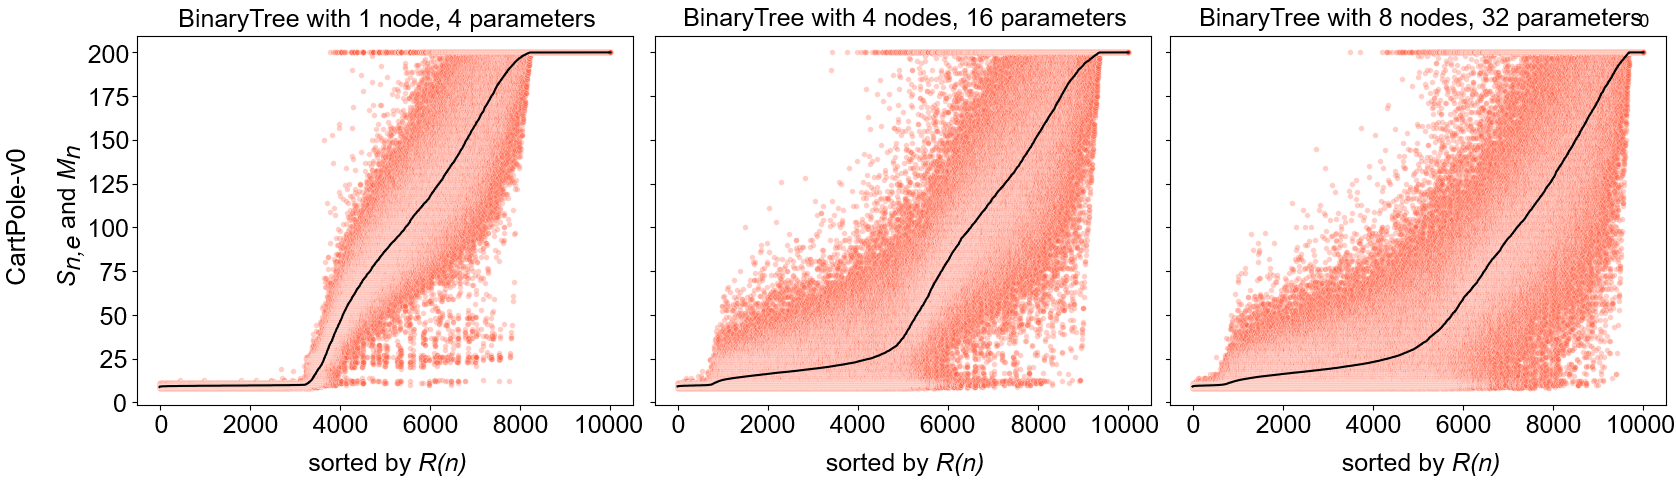
\includegraphics[width=\linewidth]{BT/BT_CartPole_new}

      \vspace{0.2cm}

  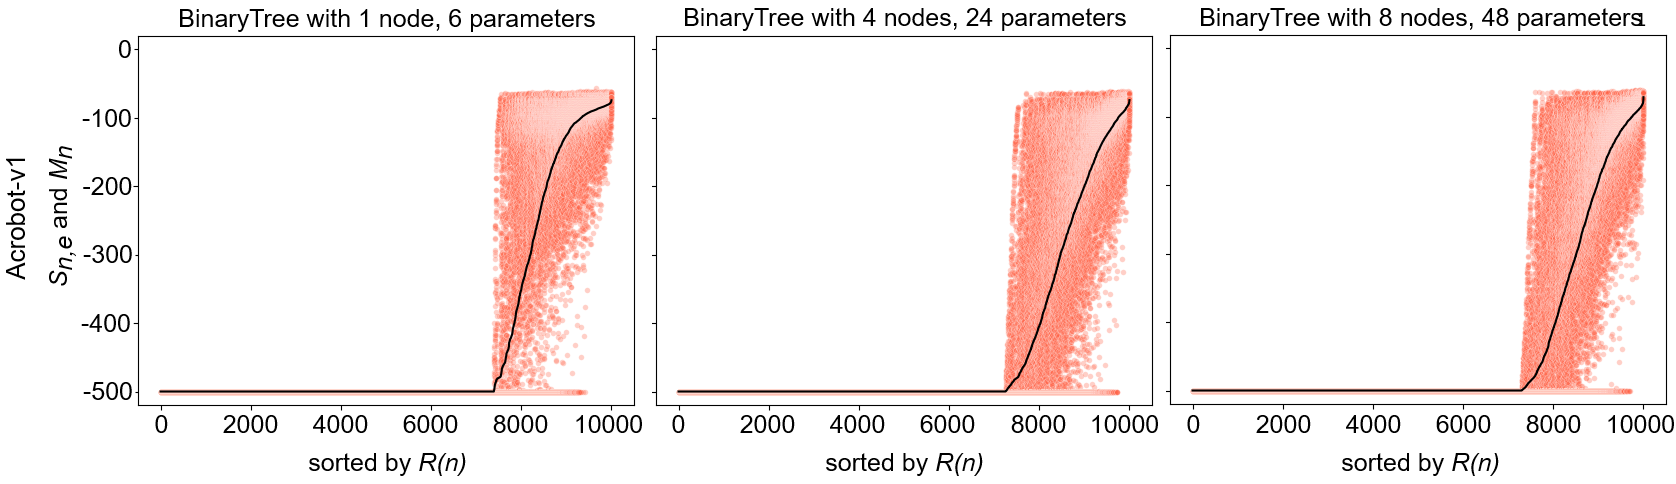
\includegraphics[width=\linewidth]{BT/BT_Acrobot_new}

      \vspace{0.2cm}

  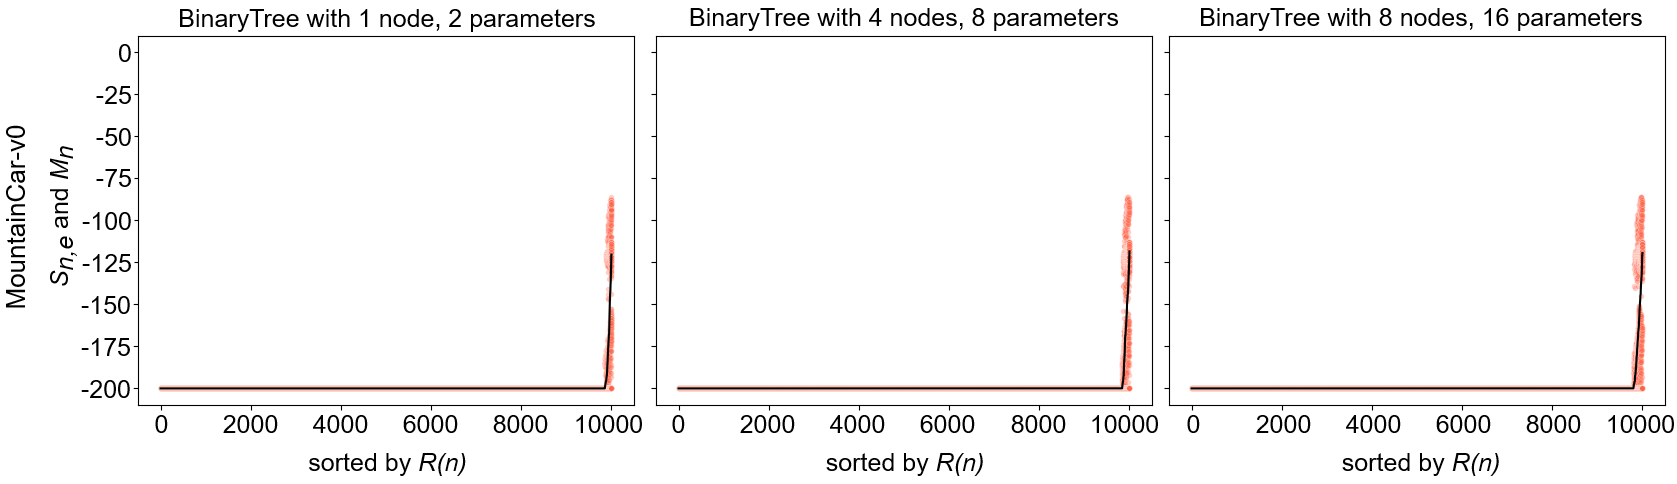
\includegraphics[width=\linewidth]{BT/BT_MountainCar_new}

      \vspace{0.2cm}

  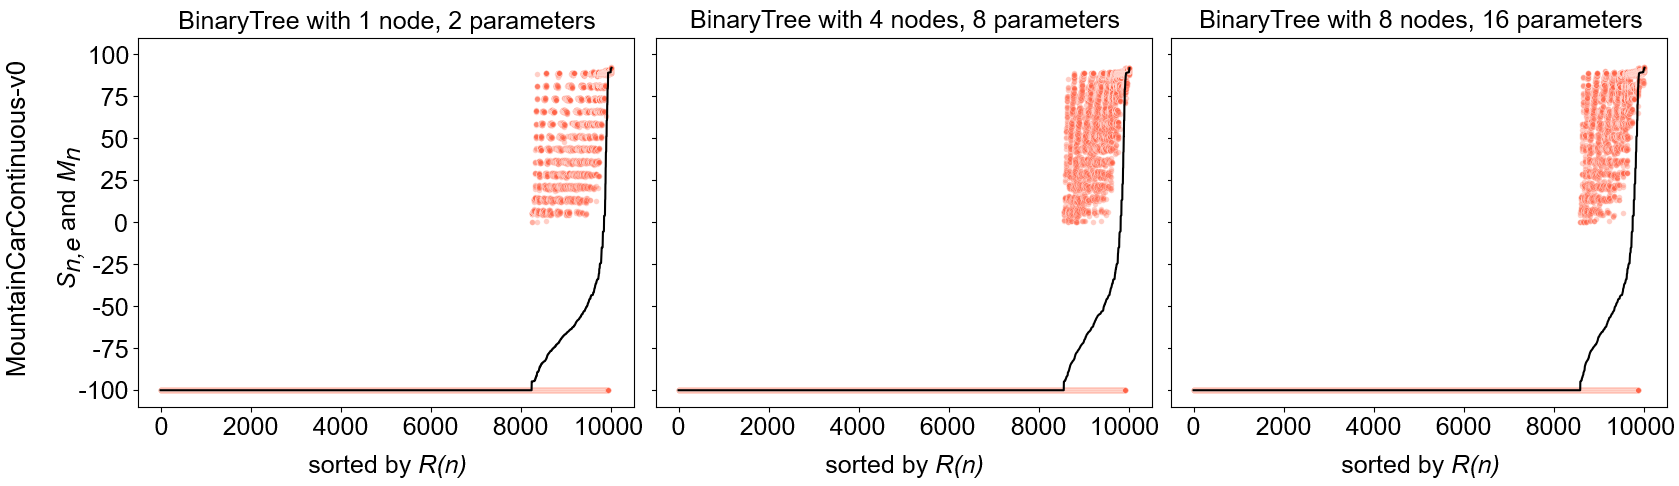
\includegraphics[width=\linewidth]{BT/BT_MountainCarContinuous_new}

      \vspace{0.2cm}

  \includegraphics[width=\linewidth]{BT/BT_Pendulum}
\caption[Results for the classic control environments using binary trees without bias]{
  \textbf{Results for the classic control environments using binary trees without bias.}
   Each row shows the results of one environment. The columns represent the different configurations for the binary tree models. Even with only one node, the results are comparable to those from neural networks or outperform them.
}
\label{fig:results_BinaryTree}
\end{figure}

\paragraph*{CartPole:} Comparing the results using binary trees with those using neural networks shown in Figure~\ref{fig:results_NN}, we can see a few differences. For the environment \verb|CartPole|, we can see that we generally reach  better scores with the binary trees. Comparing the neural network without hidden layers with the binary tree with only one node, we have a similar curve, but the lineplot representing the mean scores sets off much earlier at around 3'500 for the binary tree than the one for the neural network, which sets off at around 5'000. In addition, the binary tree has a higher chance of reaching a maximal mean score, indicated by the straight black line at the top right. For the more complex architectures, it gets more interesting.

The binary tree with four nodes can already raise the mean value under 1'000 samples. That tells us that the problem of the fitness plateau is reduced significantly. Thus, when using a learning algorithm, the binary tree has a better chance of solving the problem without getting stuck in a fitness plateau. The chance of reaching a maximal mean score decreases with adding more nodes to the binary tree. That could be caused by the increasing complexity of the binary tree, which makes it harder to guess the weights correctly. Furthermore, the scores are more spread out for the binary trees than for the neural networks, indicating a higher variance.

\paragraph*{Acrobot:} Comparing the results of the binary tree model with one node with the neural network without hidden layers for the environment \verb|Acrobot|, the binary tree produces a better score distribution. Although the fitness plateau remains to the same extent, the individual scores are overall higher, and the slope of the mean scores has improved, demonstrating a steeper slope. The neural networks with higher complexity seem to slightly outperform the binary trees with four and eight nodes. The scores are slightly higher, and the slope of the mean scores is a bit steeper. However, the difference is not massive. Overall, we can say that both models reach similar scores and mean values.

\paragraph*{MountainCar:} Comparing the two models, binary trees and neural networks, for the environment \verb|MountainCar|, we can see that they reach similar mean scores. However, the binary trees are more likely to reach more and higher individual scores. The risk of being stuck in a fitness plateau remains for the binary trees. In addition, the scores are spread wider for the binary tree than for the neural network.

\paragraph*{MountainCarContinuous:} The results for the environment \verb|MountainCarContinuous| look very different for the binary trees than for the neural networks. Neural networks show a slowly increasing curve with a peak after 9'500-9'900 samples for the mean scores. The binary trees have a lot of low performers displayed as a plateau of minimum scores. We cannot see this bad behavior in the results of the neural network models. However, there are a few samples that can reach a positive score. The neural network without hidden layers could not achieve these high mean scores.

This behavior is likely caused by the binary tree outputting discrete values instead of continuous ones, as it is the case for neural networks. The actions are fixed with the current implementation of the binary tree model. The two possible actions are the minimum and maximum of the action defined by the environment. In the case of \verb|MountainCarContiuous|, this results in either -1 or 1. However, experimenting with this action pair shows us some interesting results for the environment \verb|MountainCarContiuous|. Fiugure~\ref{fig:binary_tree_mountain_car_continuous} shows the results of using the action pair 0 and 1 instead of -1 and 1.
\begin{figure}[ht]
\centering
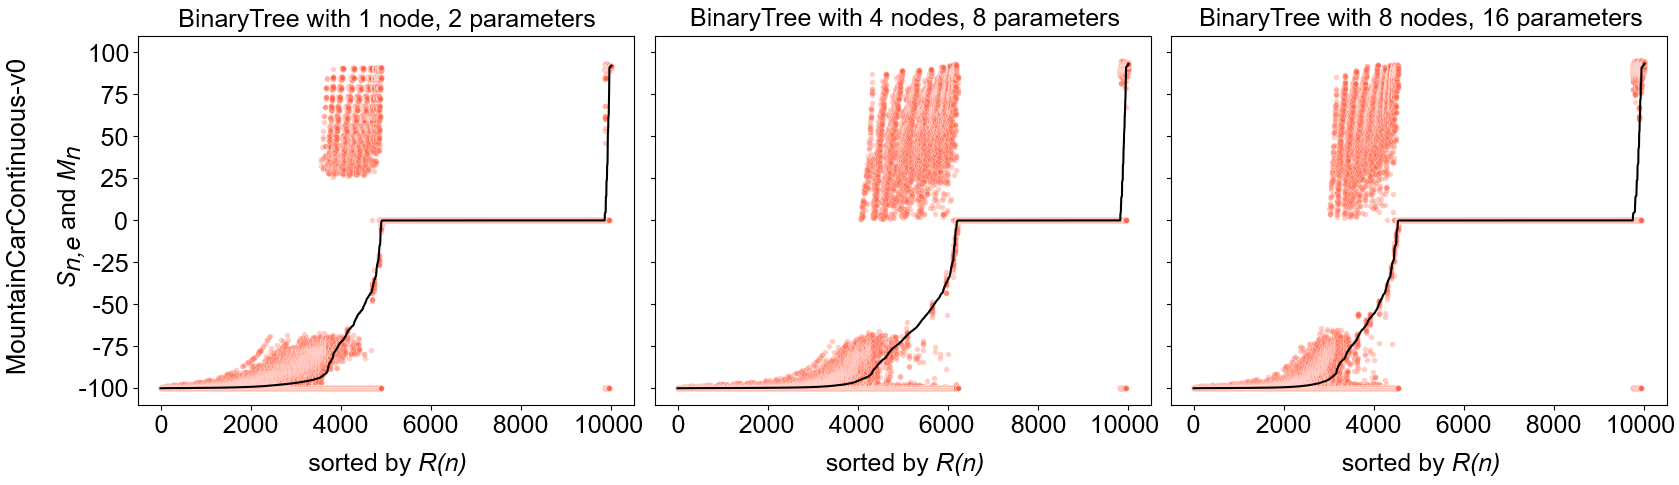
\includegraphics[width=\linewidth]{BT/BT_MountainCarContinuous_0-1_new}
\caption[MountainCarContiuous using the binary tree model with actions 0 and 1]{
  \textbf{MountainCarContiuous using the binary tree model with actions 0 and 1.}
  The figures show the results of the environment \texttt{MountainCarContiuous} using binary trees with fixed actions 0 and 1 as opposed to -1 and 1. The model's performance increased significantly compared to the results in Figure~\ref{fig:results_BinaryTree}.
}
\label{fig:binary_tree_mountain_car_continuous}
\end{figure}
There is a significant improvement in the model's performance. There are still some low performers, but the score distribution improved noticeably. However, many samples produce a zero score, resulting in a large fitness plateau.

\paragraph*{Pendulum:} For the \verb|Pendulum| environment, we can see that the binary trees perform increasingly better with more nodes. The binary tree with one node reaches a mean score of around -1'500 in the large middle area. These scores are slightly higher than those of the neural network without hidden layers in the middle area. However, the neural network reached a higher maximum mean score than the binary tree. With an increased number of nodes, the binary tree model even outperforms the neural networks with remarkably higher mean scores. Even though the actions produced by the binary trees are discrete instead of continuous, the curve of the mean scores looks very similar to the one of neural networks.

\section{Bias Investigation}
In their paper, \citet{oller_analyzing_2020} mentioned that using bias negatively affects the score distribution leading to fewer top performers and generally lower scores. Figure~\ref{fig:results_NN_bias} shows my results for all classic control environments with neural networks without using bias.
\begin{figure}
  \centering
  \includegraphics[width=\linewidth]{NN/with_bias/NN_CartPole_new}

  \vspace{0.2cm}

  \includegraphics[width=\linewidth]{NN/with_bias/NN_Acrobot_new}

  \vspace{0.2cm}

  \includegraphics[width=\linewidth]{NN/with_bias/NN_MountainCar_new}

  \vspace{0.2cm}

  \includegraphics[width=\linewidth]{NN/with_bias/NN_MountainCarContinuous_new}

  \vspace{0.2cm}

  \includegraphics[width=\linewidth]{NN/with_bias/NN_Pendulum_new}
\caption[Results for all classic control environments using neural networks with bias]{
  \textbf{Results for all classic control environments using neural networks with bias.}
   Each row shows the results of one environment, whereas the columns represent the different network architectures. For most environments, we can see that introducing a bias has a negative effect on the score distribution.
}
\label{fig:results_NN_bias}
\end{figure}
Comparing these plots with the ones without using bias in Figure~\ref{fig:results_NN}, we can see the negative impact the bias has on the effectiveness of the model. For the environment \verb|CartPole|, the scores are overall lower and get slighly worse with the increased complexity of the model. Interestingly, for the environment \verb|Acrobot|, the network without hidden layers is resistent to the negative impact of the bias. However, the network with one hidden layer results in lower scores with bias. The network with two hidden layers with has slightly better results than the one with one hidden layer but still performs worse than the one without bias. The same observation can be made for the environment \verb|MountainCar|. For the environment \verb|MountainCarContinuous|, we can see a negative effect on the score distribution for all three network architectures. The environment \verb|Pendulum| does not seem to suffer much when introducing bias. For all three architectures, there is not much difference visible. The scores are generally lower and produce less top performers when using bias. Therefore, we can confirm the interesting observation of the authors, namely, that using bias is counterproductive in this experimental setting.

\paragraph*{Altering the number of weights:} To further investigate this counterintuitive behavior, Figuer~\ref{fig:results_NN_weights} shows the results of the number of weights for the polynomial model, and Figure~\ref{fig:results_NN_weights} shows the results of tripling the number of weights for each network architecture.
\begin{figure}[!ht]
  \centering
  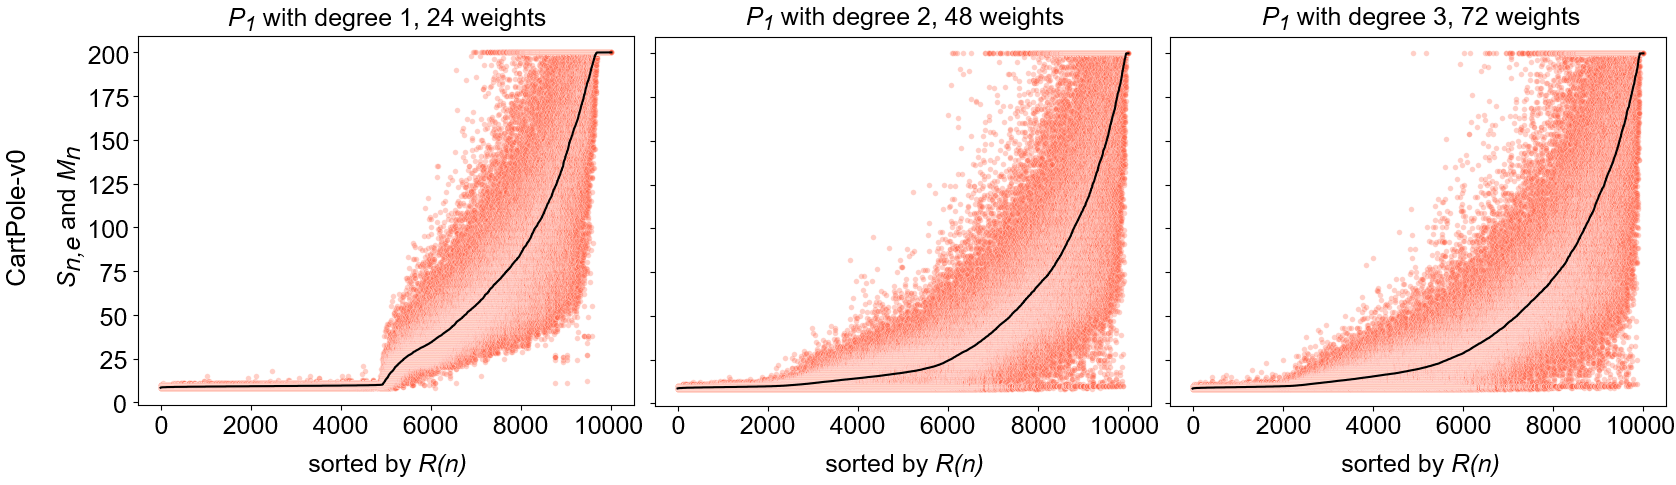
\includegraphics[width=\linewidth]{experiment_2/weights/weight_factor_3/P_CartPole_w_new}

  \vspace{0.2cm}

  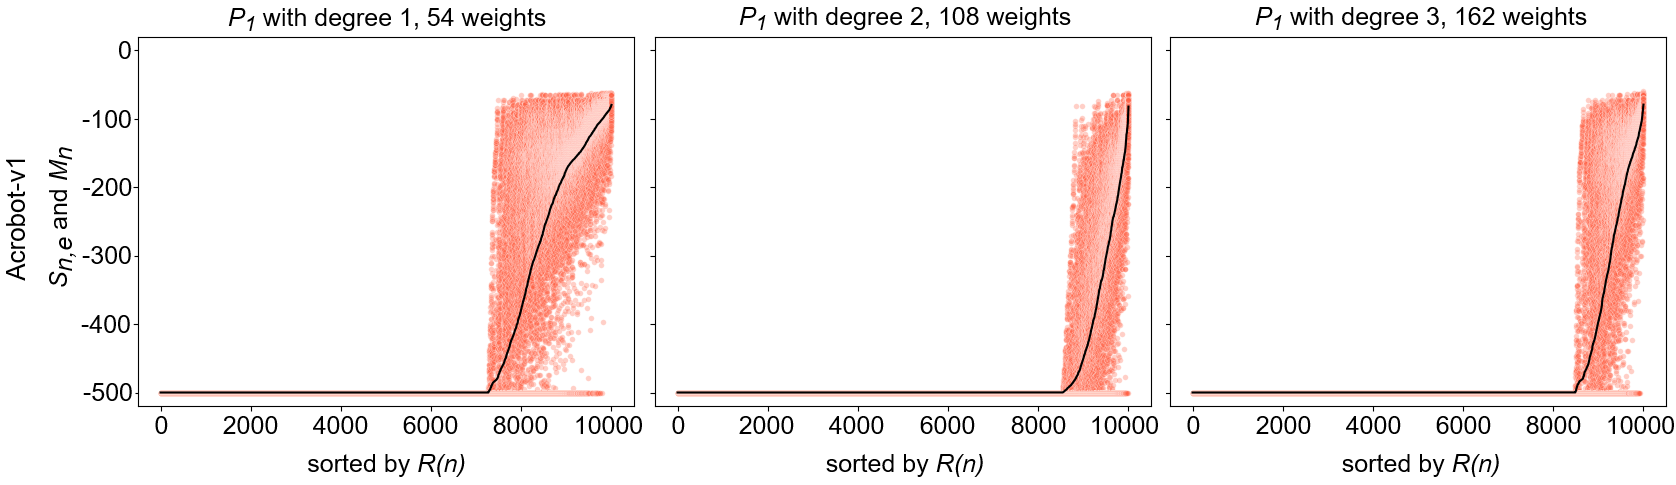
\includegraphics[width=\linewidth]{experiment_2/weights/weight_factor_3/P_Acrobot_w_new}

  \vspace{0.2cm}

  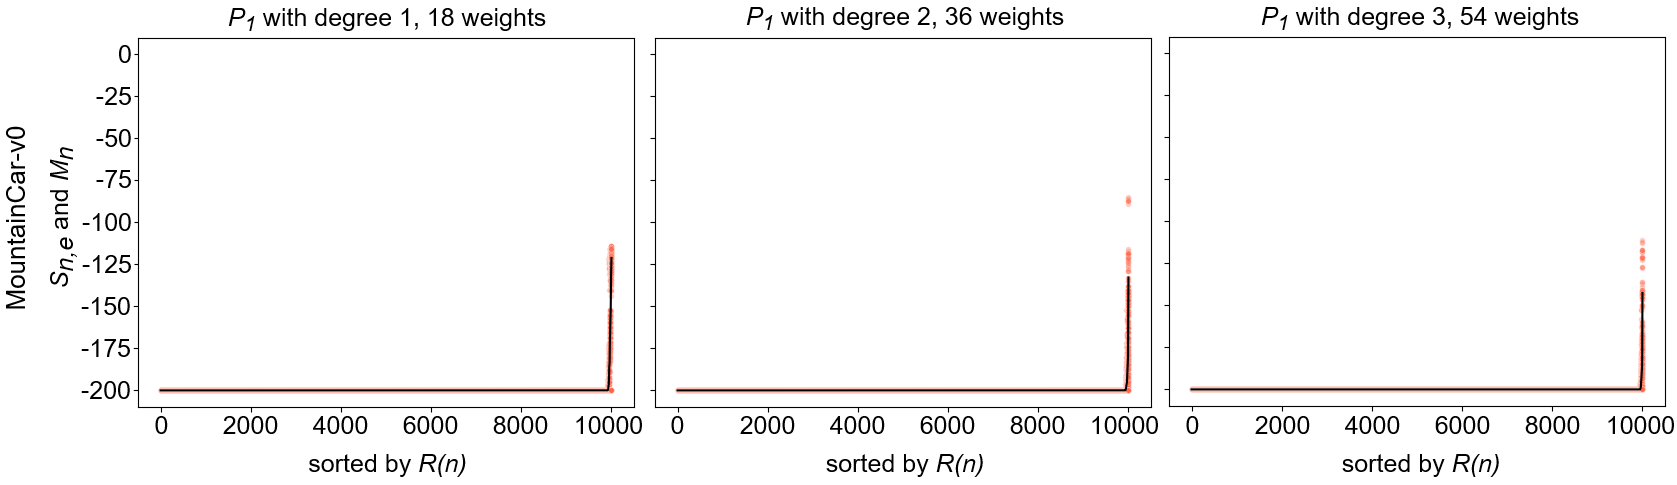
\includegraphics[width=\linewidth]{experiment_2/weights/weight_factor_3/P_MountainCar_w_new}
\caption[Results of tripling the number of weights for the poylnomial model]{
  \textbf{Results of tripling the number of weights for the polynomial model.}
   The figure shows the results of tripling the number of weights for the polynomial model for the three discrete classic control environments. Despite the increased number of weights, there are only slight differences visible in the plots of the environment \texttt{MountainCar} compared to the ones shown in Figure~\ref{fig:results_Polynomial}. \texttt{Acrobot} and \texttt{CartPole} look indistinguishable from the other results.
}
\label{fig:results_NN_weights}
\end{figure}
Comparing the results of the polynomial models, we cannot see a difference for the environments \verb|CartPole| and \verb|Acrobot| comparing these results with those shown in Figure~\ref{fig:results_Polynomial}. The environment \verb|MountainCar| shows only slight differences.

Comparing the plots in Figure~\ref{fig:results_NN_weights} to those in Figure~\ref{fig:results_NN}, we cannot see a huge difference. The score distribution of the environments \verb|CartPole| and \verb|Acrobot| look indistinguishable from those presented in Figure~\ref{fig:results_NN}.
\begin{figure}
  \centering
  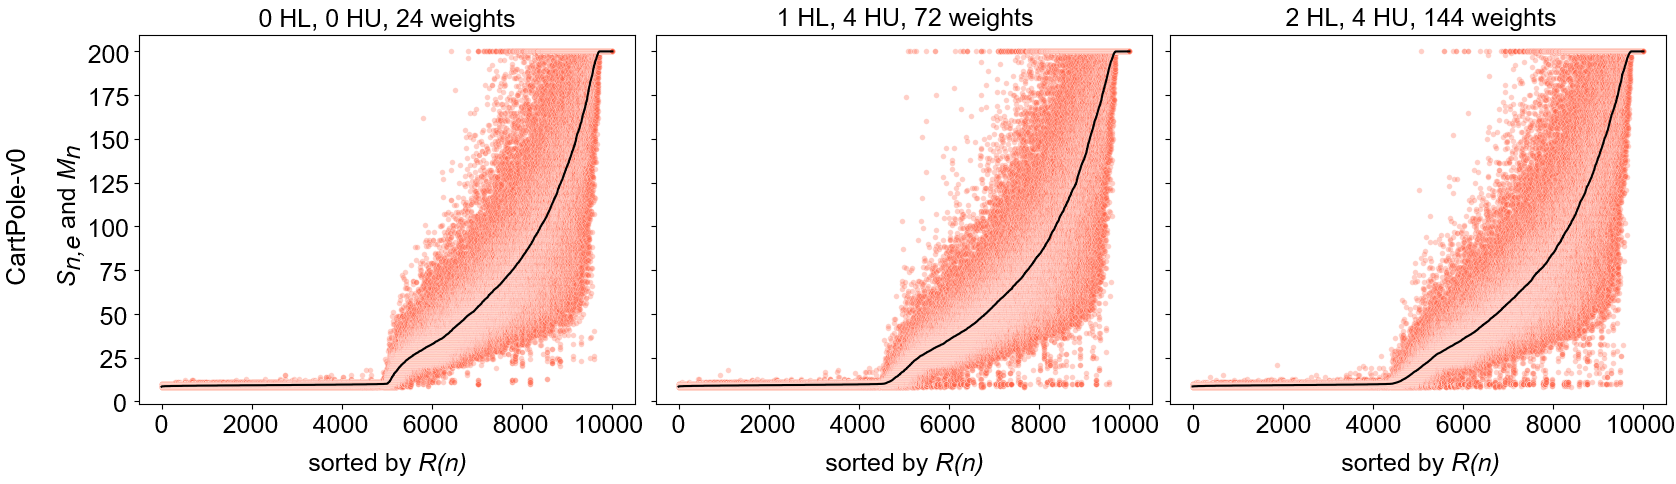
\includegraphics[width=\linewidth]{experiment_2/weights/weight_factor_3/NN_CartPole_w_new}

  \vspace{0.2cm}

  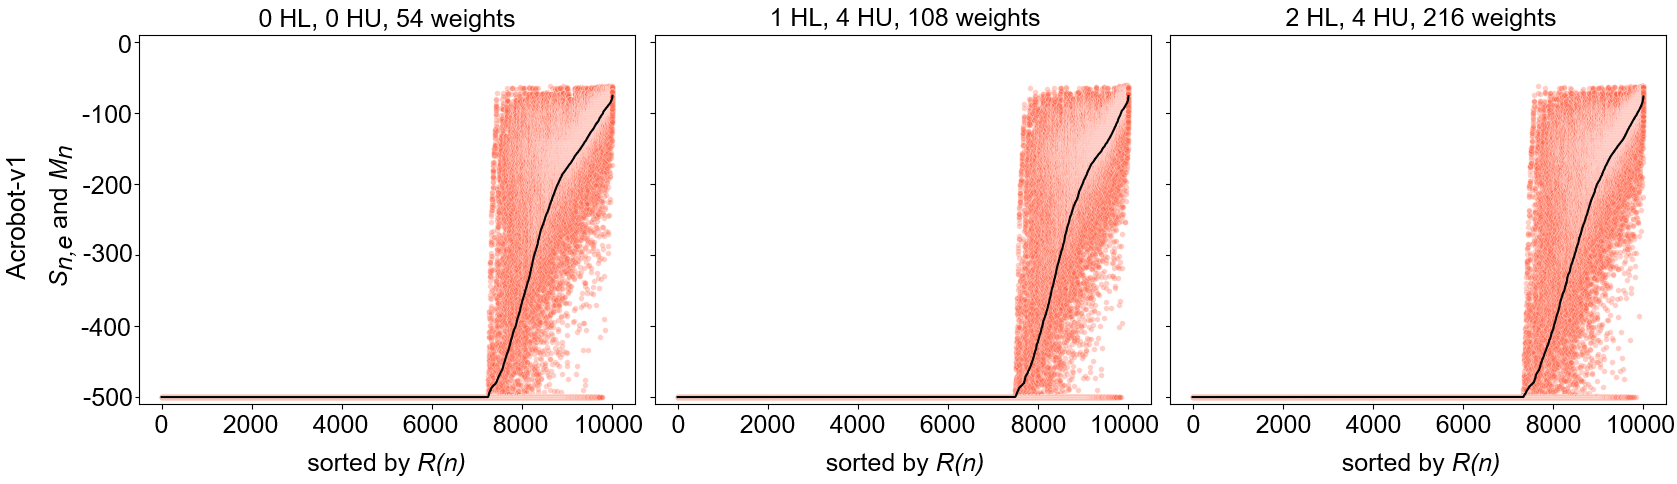
\includegraphics[width=\linewidth]{experiment_2/weights/weight_factor_3/NN_Acrobot_w_new}

  \vspace{0.2cm}

  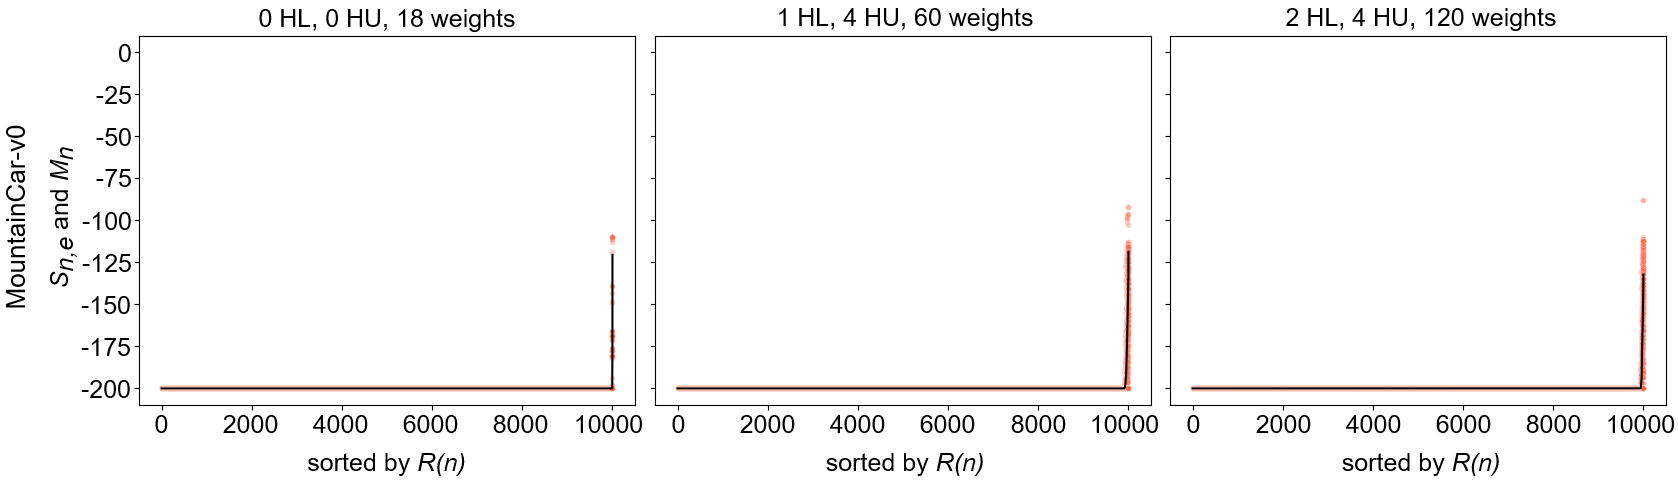
\includegraphics[width=\linewidth]{experiment_2/weights/weight_factor_3/NN_MountainCar_w_new}

  \vspace{0.2cm}

  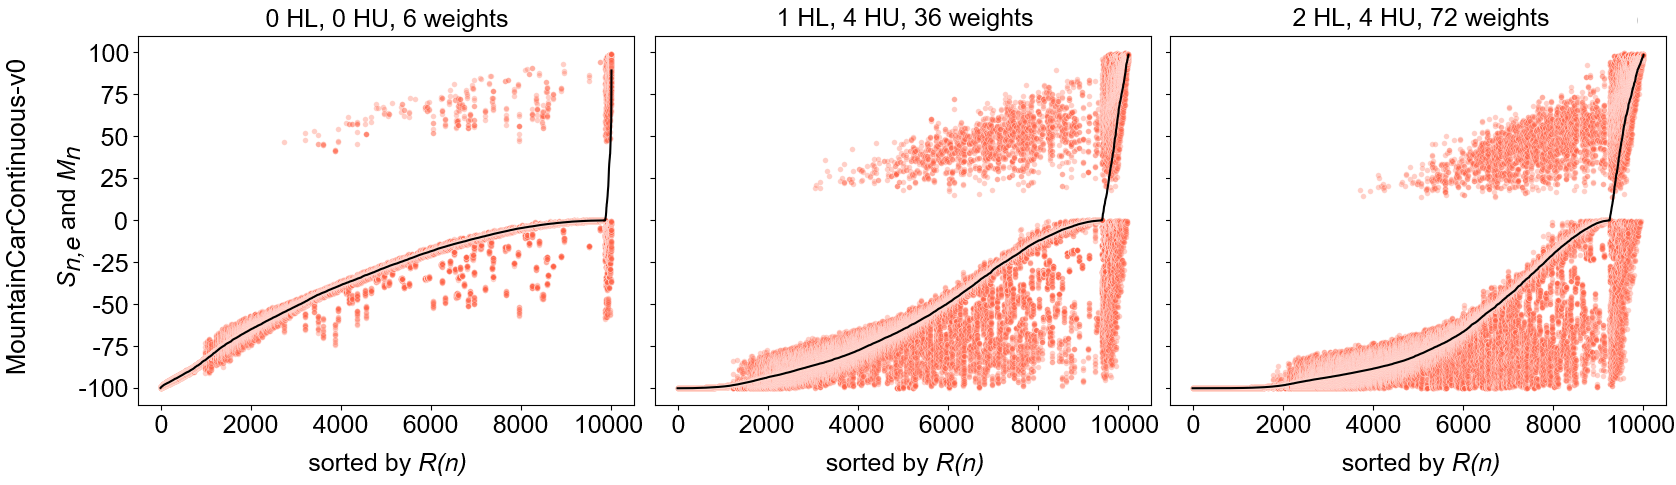
\includegraphics[width=\linewidth]{experiment_2/weights/weight_factor_3/NN_MountainCarContinuous_w_new}

  \vspace{0.2cm}

  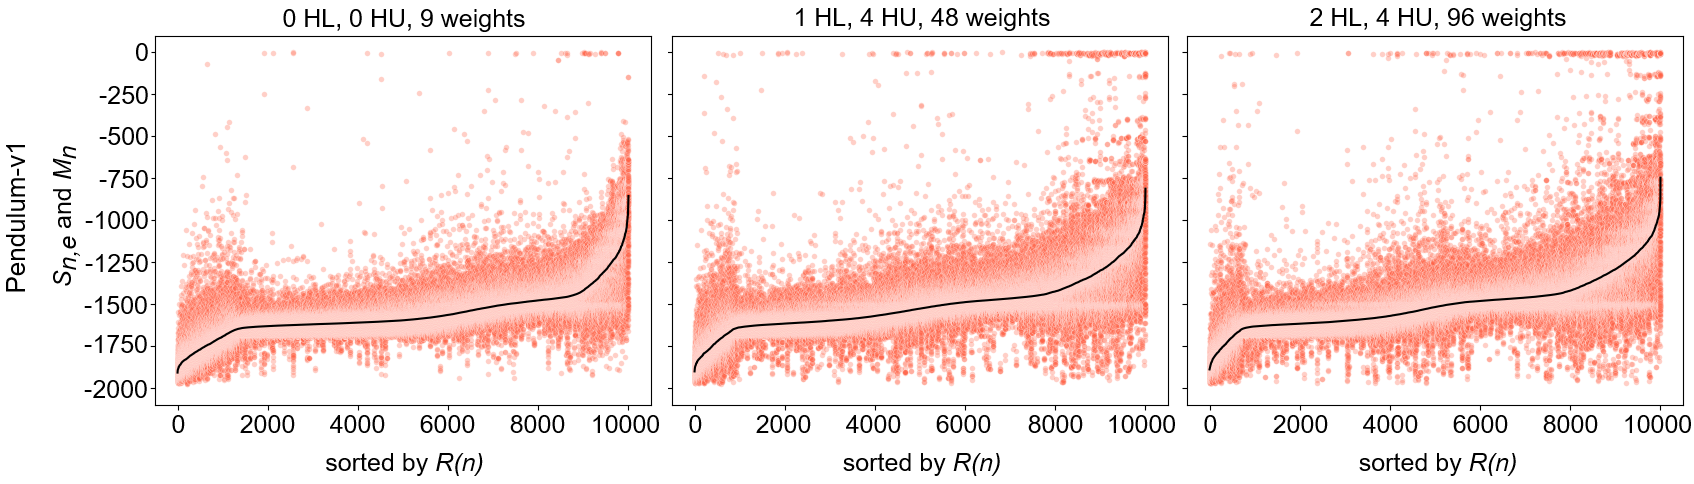
\includegraphics[width=\linewidth]{experiment_2/weights/weight_factor_3/NN_Pendulum_w_new}
\caption[Results of tripling the number of weights for neural networks]{
  \textbf{Results of tripling the number of weights for neural networks.}
   The figure shows the results of tripling the number of weights for the three neural network architectures for the classic control environments. Despite the increased number of weights, there are only slight differences visible in the plots compared to the ones shown in Figure~\ref{fig:results_NN} for all environments with the exception of \texttt{MountainCarContinuous}.
}
\label{fig:results_NN_weights}
\end{figure}
We can see slight differences in the plots for the environment \verb|MountainCar|. Increasing the number of weights for the network without hidden layers results in a few better individual scores without much difference in the mean score distribution. We see slightly better mean scores for the network with one hidden layer, whereas the network with two exhibits slightly worse mean scores. For the environment \verb|MountainCarContinuous|, the mean scores are lower compared to the networks with more weights. However, there are more top performers.  This is especially visible for the network without hidden layers.

In addition, the scores are more spread out. There are a few more samples that reach a higher score for the environment \verb|Pendulum| with the network without hidden layers. However, the networks with one and two hidden layers deliver similar results to those shown in Figure~\ref{fig:results_NN} for the environment \verb|Pendulum|. To summarize, altering the number of weights for a network can produce a slight difference in the results for some environments. But these differences are not as dramatic as we have seen for the networks without using bias.

\paragraph*{Altering the number of layers:} Figure~\ref{fig:experiment_2_layers} shows the results of altering the number of layers in a network.
\begin{figure}
  \centering
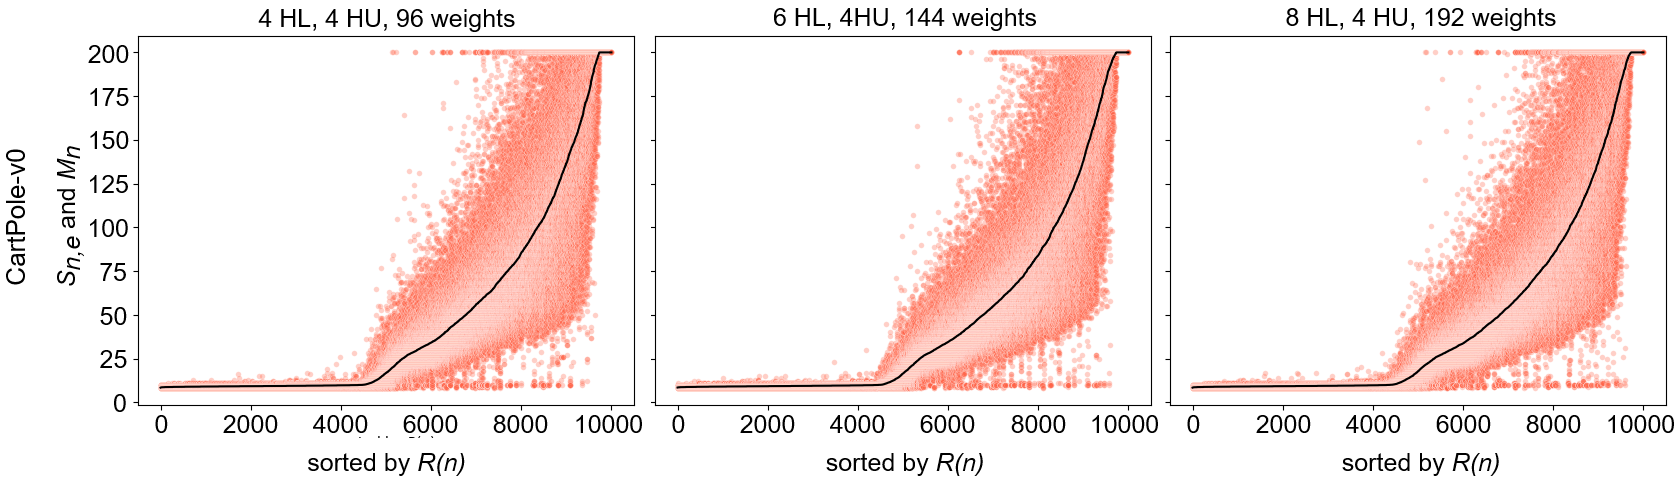
\includegraphics[width=\linewidth]{experiment_2/layers/NN_CartPole_l_new}

  \vspace{0.2cm}

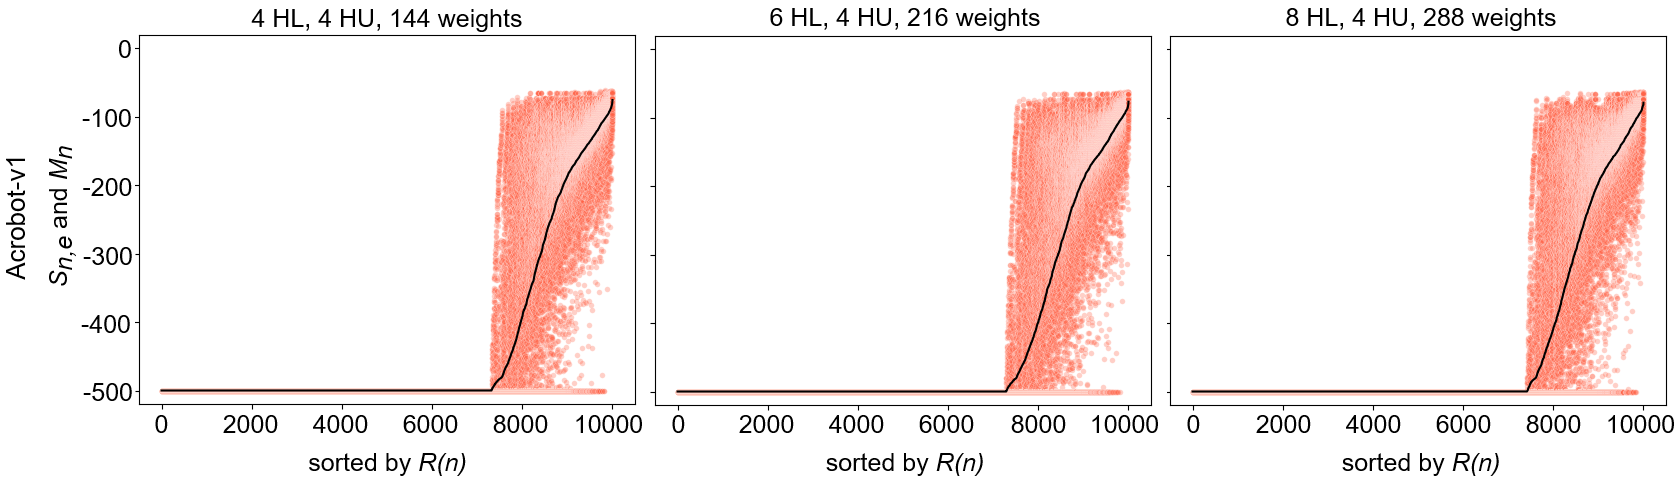
\includegraphics[width=\linewidth]{experiment_2/layers/NN_Acrobot_l_new}

  \vspace{0.2cm}

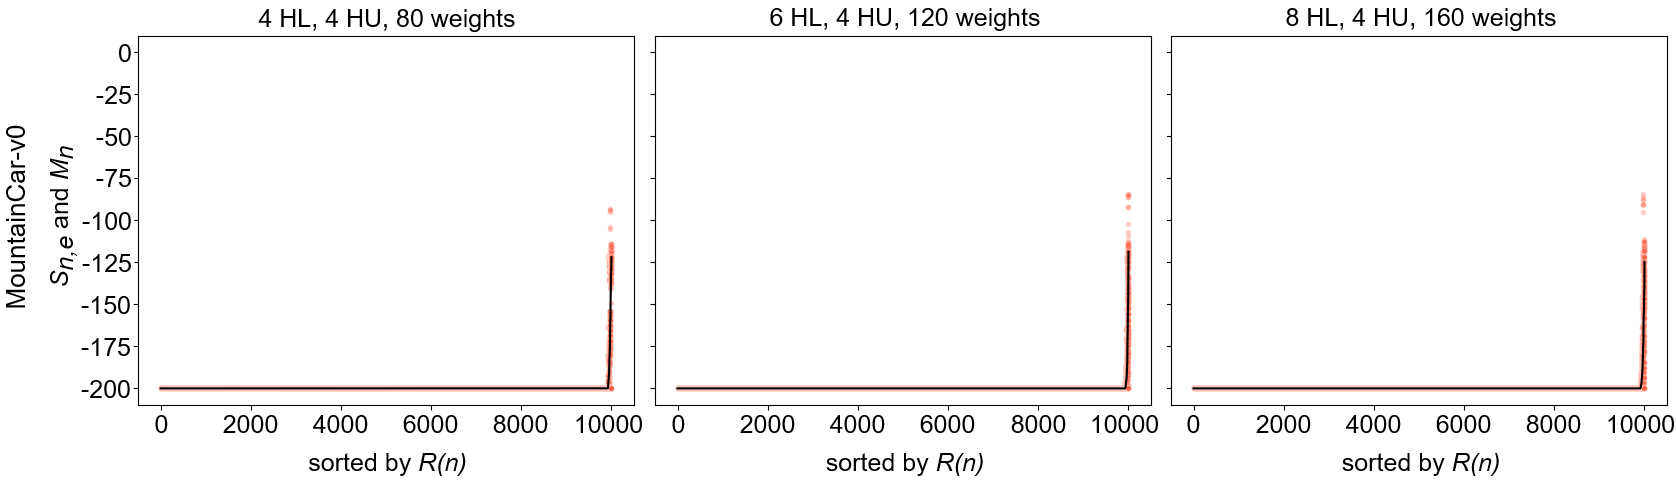
\includegraphics[width=\linewidth]{experiment_2/layers/NN_MountainCar_l_new}

  \vspace{0.2cm}

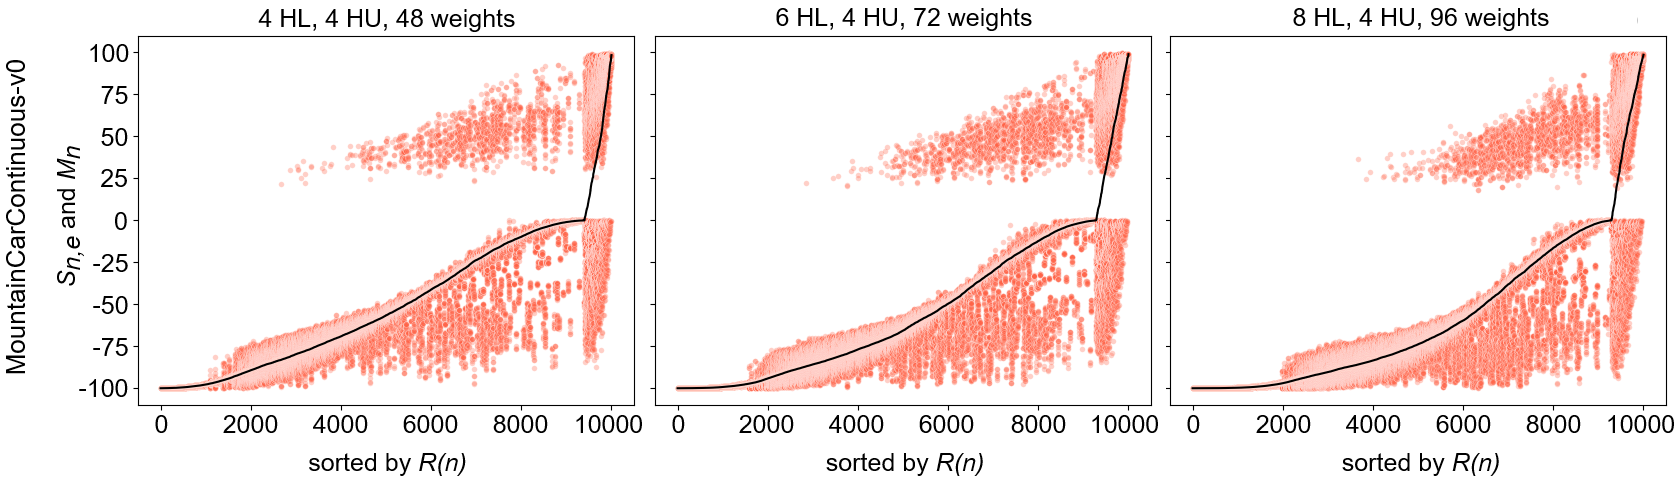
\includegraphics[width=\linewidth]{experiment_2/layers/NN_MountainCarContinuous_l_new}

  \vspace{0.2cm}

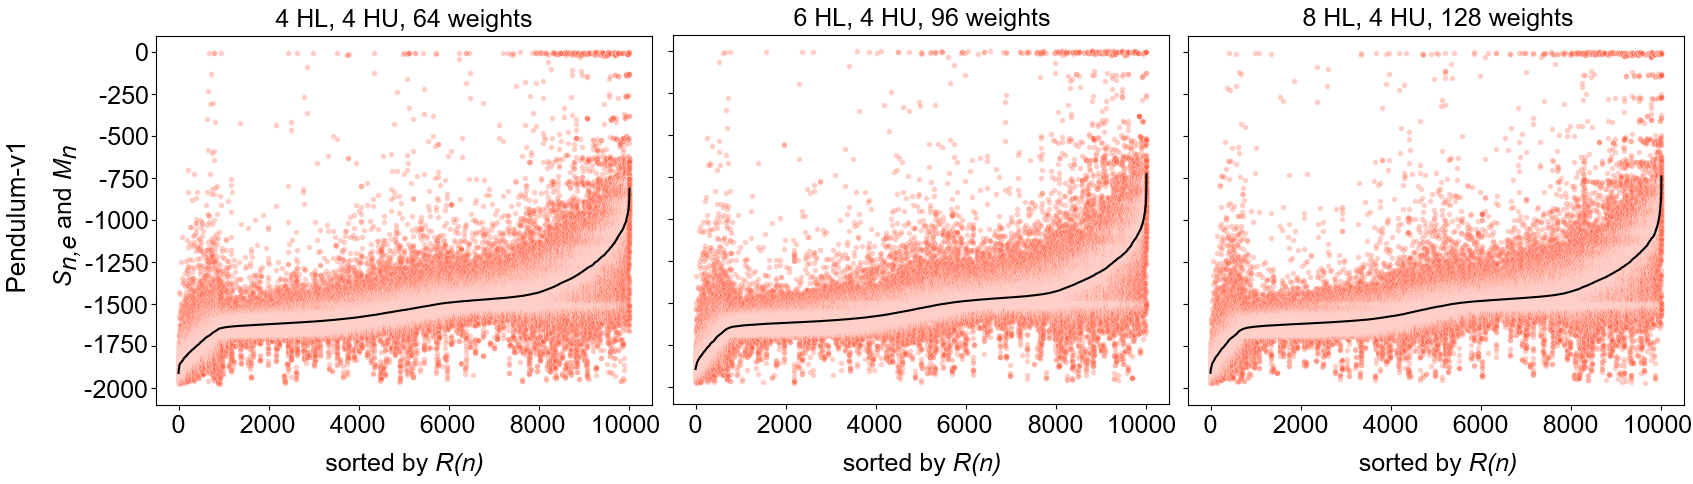
\includegraphics[width=\linewidth]{experiment_2/layers/NN_Pendulum_l_new}
\caption[Results of altering the number of layers for neural networks]{
  \textbf{Results of altering the number of layers for neural networks.}
   The plots show the results of increasing the number of hidden layers in a neural network gradually. The score distribution changes with an increased number of layers for some environments. However, the changes are less extreme compared to the results of the networks that used bias.
}
\label{fig:experiment_2_layers}
\end{figure}
Each layer still has the same amount of neurons, namely four neurons. For the environment \verb|CartPole|, the lineplot of the mean scores seems to start earlier to rise above the minimum score, but the slope is also slightly less steep with an increasing number of hidden layers. The environment \verb|Acrobot| does not seem to be affected anyhow by the change in the number of layers. The plots look indistinguishable. The mean scores for the environment \verb|MountainCar| seem to be best for the network with four hidden layers. The scores tend to get lower with an increased number of layers. For the environment \verb|MountainCarContinuous|, the slope of the mean scores changes. The scores get generally slightly lower with more layers. Finally, we cannot see a big difference in the plots for the environment \verb|Pendulum| by adding more layers. There may be a few more top performers with more hidden layers, but the difference is not significant and is not reflected in the mean score distribution.

\paragraph{Altering the number of neurons:} Figure~\ref{fig:experiment_2_neurons} shows the results of increasing the number of neurons in each hidden layer for a network with two hidden layers.
\begin{figure}[!ht]
  \centering
  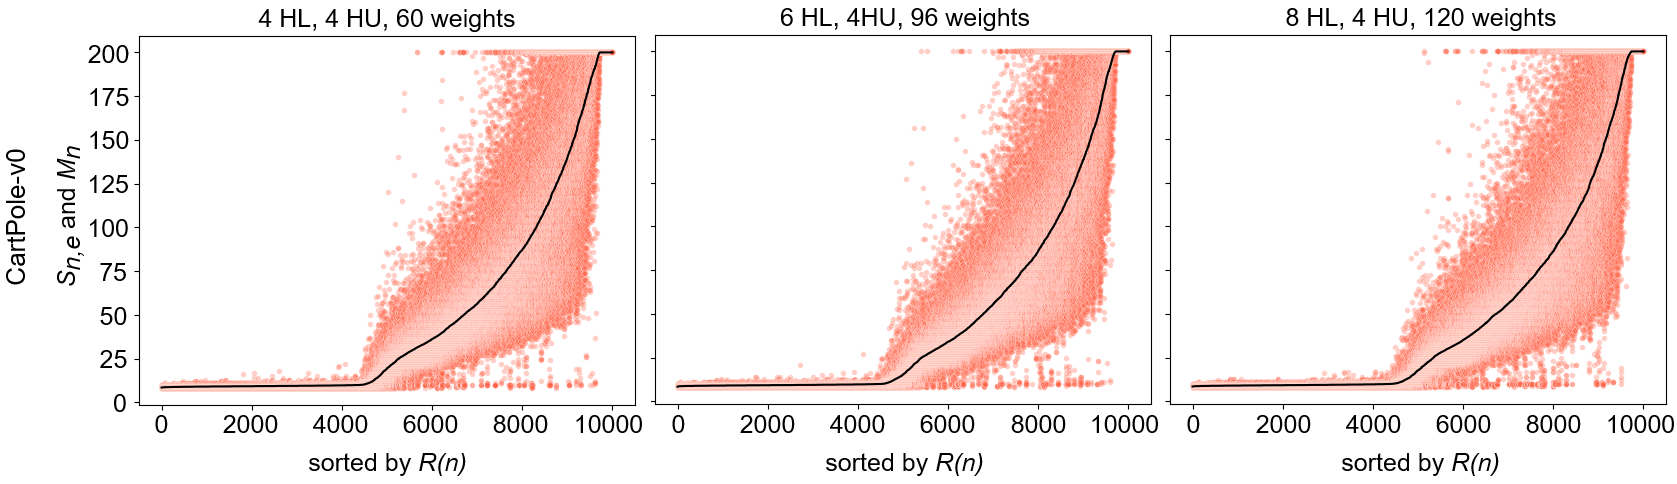
\includegraphics[width=\linewidth]{experiment_2/neurons/NN_CartPole_n_new}

    \vspace{0.2cm}

  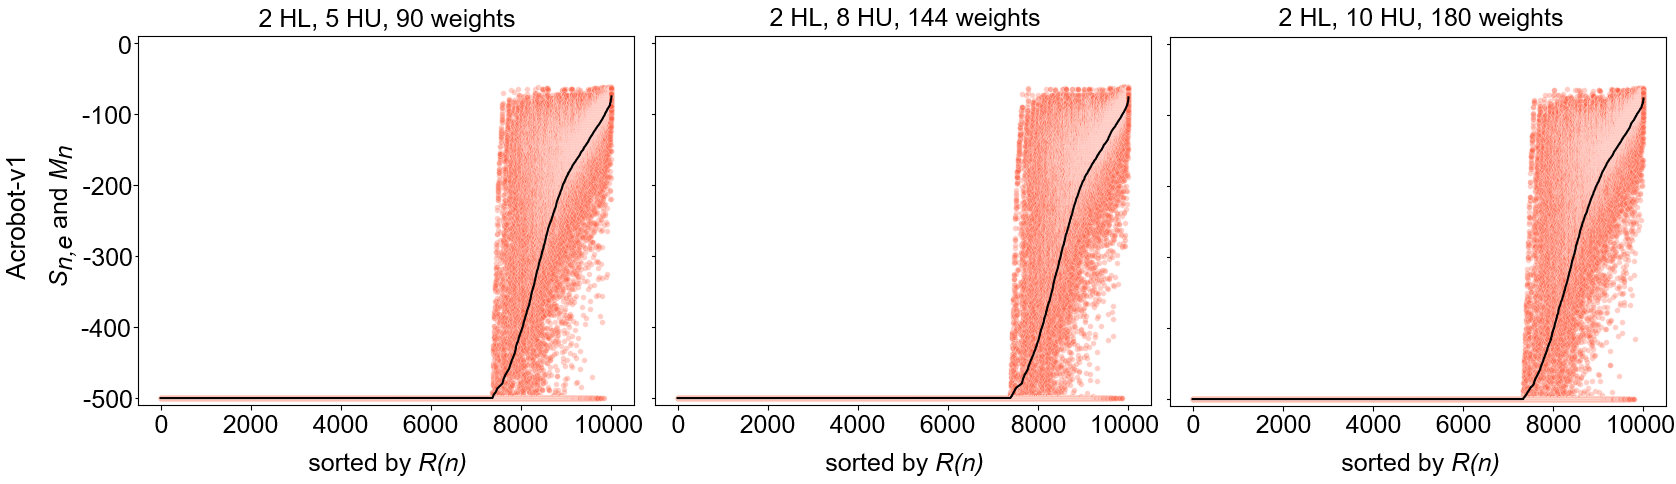
\includegraphics[width=\linewidth]{experiment_2/neurons/NN_Acrobot_n_new}

    \vspace{0.2cm}

  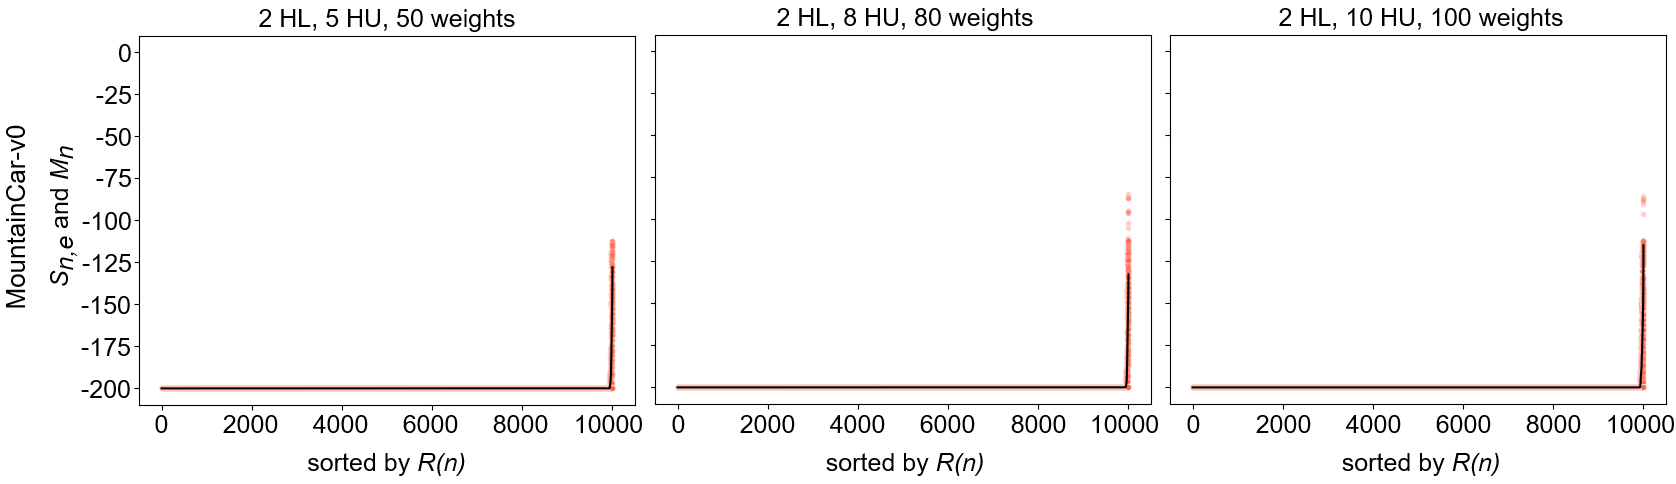
\includegraphics[width=\linewidth]{experiment_2/neurons/NN_MountainCar_n_new}

    \vspace{0.2cm}

  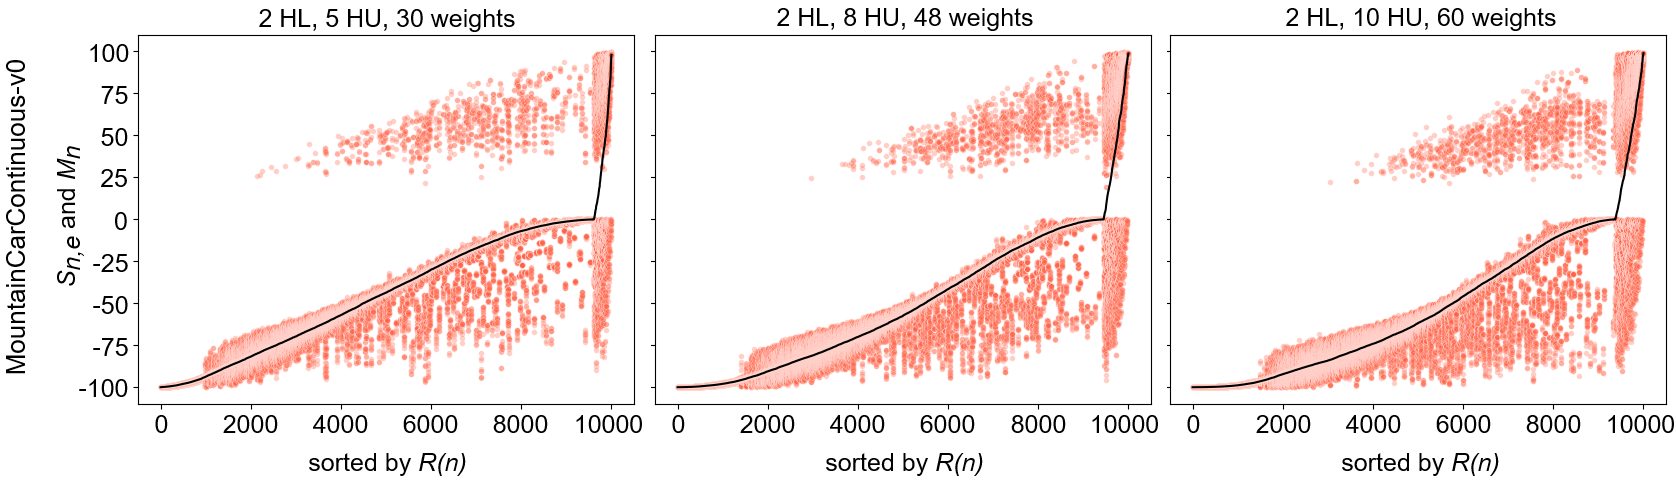
\includegraphics[width=\linewidth]{experiment_2/neurons/NN_MountainCarContinous_n_new}

    \vspace{0.2cm}

  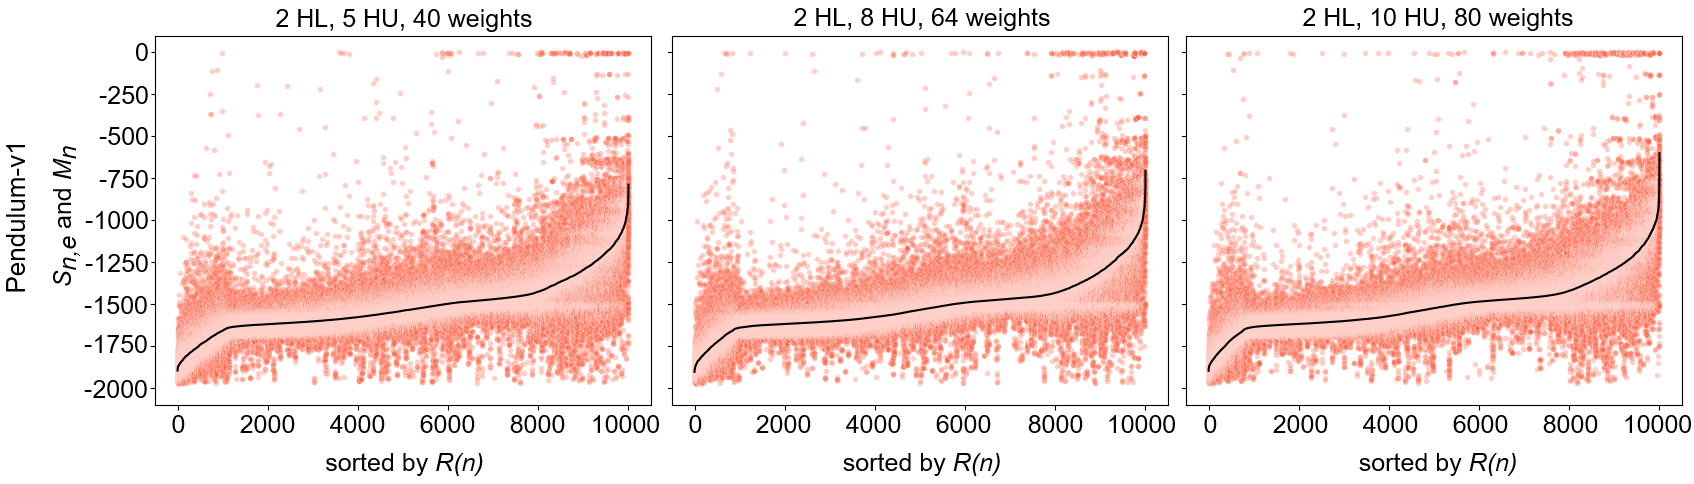
\includegraphics[width=\linewidth]{experiment_2/neurons/NN_Pendulum_n_new}
\caption[Results of altering the number of neurons for neural networks]{
  \textbf{Results of altering the number of neurons for neural networks.}
  The plots show the result of increasing the number of neurons for each layer in a network with two hidden layers. For some environments, there is a change in the mean scores. However, the changes are not extreme.
}
\label{fig:experiment_2_neurons}
\end{figure}
We cannot see much difference in the plots for the environments \verb|CartPole| and \verb|Acrobot|. For both, the score distribution seems to be unaffected by the increased number of neurons. The mean scores for the environment \verb|MountainCar| first decrease with five and eight neurons. Then with ten neurons, we achieve higher scores again. For the environment \verb|MountainCarContinuous|, the plots look similar to the ones in Figure~\ref{fig:experiment_2_layers} with an increased number of layers. We can see a slight decrease in the scores with increased neurons which is less extreme than when we increased the number of layers. With the environment \verb|Pendulum|, we can reach higher mean scores with an increased number of neurons. Otherwise, the slope of the mean scores and the overall score distribution looks very similar.

\clearpage
\section{Discussion}
This chapter delivered a direct comparison between neural networks and alternative models: polynomials and binary trees. In addition, I investigated the impact of bias in these settings. The subsequent paragraphs aim to discuss the results to prepare for the conclusions and proposed future work in the next chapter.

\paragraph*{Comparison of polynomial model with neural networks:} As we have seen in the last section, the polynomial model can deliver comparable results to neural networks for discrete environments. The results of the environment \texttt{MountainCar} with the polynomial model look almost indistinguishable from those of the neural network model. For the environment \texttt{Acrobot} the polynomial model with degree delivers very similar results as the neural network without hidden layers. With the higher complexity of the model, neural networks outperform the polynomial model.

The polynomial of degree one results in the same score distribution as the neural network without hidden layers. The score distribution differs noticeably from neural networks with higher model complexity. The mean scores show the same trend for all neural network architectures, which cannot be applied to the polynomial model.

With the linear polynomial model, we have a $50 \%$ chance of failing, but the probability of actually solving the task for all episodes is higher than for the polynomials with a higher degree. That means with the linear model or neural networks, we have a larger fraction of samples that can solve the environment independently of the initialization conditions. We could assume that this is an important aspect for such a model and choose the polynomial with degree 1 over one with a higher degree. We should remind ourselves that these experiments are rather unusual for an application since there is no learning involved and the number of samples is huge.

In a standard application, we would use some kind of training and want the model to sequentially improve its performance. When using a learning algorithm, we would not prefer the polynomials with degree one or the neural networks as we might get stuck in a fitness plateau when the algorithm has no method of dealing with this behavior.

The results of the polynomial model are comparable to those of neural networks. This applies only for the three discrete environments since the polynomial model is not constructed to deal with a continuous action space.

\paragraph*{Comparison of binary tree model with neural networks:} Despite the simple structure of the binary tree model, it delivers comparable results to neural networks and even outperformed them. The binary tree model significantly outperforms neural networks for the environment \verb|CartPole| for all three architectures. The binary tree with only one node shows a similar slope for the mean scores as the network without hidden layers, but it visibly reduces the plateau of minimum scores. The binary trees with higher complexity even manages to remarkably shrink the plateau, which none of the three architectures of the neural network did on that scale.

The environment \verb|MountainCar| yields similar mean scores for the binary trees and the neural networks. There is a large plateau of minmum scores for both models. When comparing the three configurations of the two models with each other, we can see that the binary tree model reaches more and higher individual scores than the neural network models. The results of the two models are similar for the two models for the environment \verb|Acrobot|. The binary tree with one node outperforms the neural network without hidden layers whereas the complexer neural networks outperform the binary trees with four and eight nodes.

Even though the binary tree model at its current implementation outputs only discrete action values, the results for the continuous environment \verb|Pendulum| are comparable to those of neural networks. The binary tree with eight nodes even managed to outperform neural networks. For the environment \verb|MountainCarContinuous|, neural networks delivered better results. Although the binary tree model with one node reached significantly higher mean scores than neural networks, it exhibits a large plateau of minimum scores that we do not see for the neural networks. The networks with higher complexity reached identical high mean scores.

The considerable difference in the score distribution between the two models could be caused by the binary tree producing discrete actions instead of continuous ones, as neural networks did. For the binary tree model, the action is either -1 or 1, limiting the output space significantly. The environment \verb|MountainCarContiuous| seems more sensitive to these discrete action outputs than the environment \verb|Pendulum|. The experiments with the choice of actions resulted in a much better score distribution for the action pair 0 and 1.

The binary tree model produced a similar score distribution as neural networks did. For some environments, the binary trees even outperform neural networks. The environment \verb|MountainCarContinuous| seems more difficult for the binary trees to learn than for neural networks.

\paragraph*{Impact of bias:} Including bias has a significant negative impact on almost all of the five classic control environments. For the environment \verb|Acrobot| and \verb|Pendulum|, the difference between using bias and not using bias seems less extreme than for the other environments depending on the number of layers used.

To further investigate this behavior, I subsequently changed three aspects of the model's architecture. First, I increased the number of weights of the networks. Despite the remarkably increased number of weights, the results show only slight differences in the score distribution. The exception is the environment \texttt{MountainCarCon-} \texttt{tinuous}, where the mean scores are remarkably lower. Except for the environment \texttt{MountainCarContinuous}, we can conclude that the increased number of weights does not impact the score distribution significantly.

Second, I increased the number of hidden layers. Some environments show slightly different results like \verb|CartPole| and \verb|MontainCar|. However, the changes are less significant than in the experiments with bias connections. The exception is again \verb|MountainCarContinuous|, where the difference is noticeably more extreme with an increased number of layers.

Finally, I increased the number of neurons in each hidden layer. In the results of this experiment, some changes in the score distribution are visible. The mean scores of the environments \verb|Pendulum| and \verb|MountainCar| show slight differences. The environment \verb|MountainCarContinuous| shows a similar picture as before.

In summary, no other aspect impacts the performance of the model as negative as using bias. The exceptions are the environment \verb|MountainCarContinuous|, where we see even more extreme differences when changing the network architecture, and \verb|Pendulum|, which already shows smaller differences than the other environments when using bias versus not using bias. It seems that this behavior is specific to the bias in the setting of RWG for the environments \verb|CartPole|, \verb|Acrobot|, and \verb|MountainCar|. In addition, we have seen that the environment \verb|MountainCarContinuous| generally reacts sensitive to a change in the model's architecture, showing a similar image as when using bias. In contrast, \verb|Pendulum| does not seem to be significantly affected by a change in the architecture. But as we have seen, the bias also affects it less.
